\documentclass[12pt,a4paper]{article}
\renewcommand{\baselinestretch}{1.5} 
% inputenc removed to ensure compatibility with modern LuaTeX/XeTeX compilers
\usepackage{amsmath}
\usepackage{amsfonts}
\usepackage{amssymb}
\usepackage{algorithm} 
\usepackage{algpseudocode} 
\usepackage{graphicx}
\usepackage{geometry}
\usepackage{tabulary}
\usepackage{caption}
\usepackage{subcaption}
\usepackage{xcolor}
\usepackage{dirtytalk}
\usepackage{bm}
\usepackage{longtable}
\usepackage{comment}
\usepackage{listings}
\usepackage{booktabs}
\usepackage{float}
\graphicspath{{./images/}}

\usepackage[hyphens]{url}

\geometry{
	left=2.5cm,
	right=2.5cm,
	top=2.5cm,
	bottom=3cm,
}

\usepackage{titlesec}

\setcounter{secnumdepth}{4}
\setcounter{tocdepth}{4}
\titleformat{\paragraph}
{\normalfont\normalsize\bfseries}{\theparagraph}{1em}{}
\titlespacing*{\paragraph}
{0pt}{3.25ex plus 1ex minus .2ex}{1.5ex plus .2ex}

\newenvironment{conditions}
{\par\vspace{\abovedisplayskip}\noindent\begin{tabular}{>{$}l<{$} @{${}={}$} l}}{\end{tabular}\par\vspace{\belowdisplayskip}}

% Code listing style
\lstset{
  basicstyle=\ttfamily\small,
  breaklines=true,
  frame=single,
  columns=fullflexible
}

% Fallback title definitions in case titlepage.tex is missing
\title{\textbf{Stochastic Block Jacobi Page-Rank Acceleration}}
\author{Technical Report}
\date{}

\begin{document}
    % Safely include titlepage if it exists, otherwise use fallback
    \IfFileExists{titlepage.tex}{
        \thispagestyle{empty}
\begin{center}
	{\Large \bf Stochastic Block Jacobi Page-Rank Acceleration\\}
	
	\vspace*{0.5cm}
	{\large\textit{A Project Component for }\\}
	%\vspace*{0.3cm}
	{\large\textbf{Parallel and Distributing Computing (UCS645)}} \\
%	{\large in\\}
%	{\large \textbf{CSED} }
	
	%\vspace*{1cm}
	{\large \textit{By\\}}
	\textbf{\begin{table}[h!]
\label{tab:my-table}
\centering
\begin{tabular}{ccc}
Sr & Name     & Roll No  \\
1  & Mannat   & 102303148 \\
2  & Lavisha  & 102303423 \\
3  & Nikhil   & 102303512 \\
4  & Shrestha & 102303878 \\
\end{tabular}
\end{table}}
% update the name of the students based on number
	%\vspace*{0.5cm}
		\begin{center}
                {\large \textit{Under the guidance of}}\\
					\textbf{{\large Dr. Saif Nalband}}\\
					{\large (Assistant Professor, DCSE)}\\
		\end{center} \ \\ \ \\
\begin{figure}[h]
\centering
\includegraphics[width=70mm, height=40mm]{"tietlogo.jpg"}
\label{fig:images}
\end{figure}

%	in case the layout changes modify the below vspace 1.25 and appropiately make sure that title page is contained in one single page	
	\vspace*{0.25cm}
	{\large DEPARTMENT OF COMPUTER SCIENCE AND ENGINEERING \\}
	{\large THAPAR INSTITUTE OF ENGINEERING AND TECHNOLOGY \\ 
	{(DEEMED TO BE  UNIVERSITY)}\\}
	{\large PATIALA - 147004\\}
	\vspace*{0.3cm}
	\textbf{{\large MAY, 2026}}
	
\end{center}

\newpage
    }{
        \maketitle
        \thispagestyle{empty}
    }
%%%%%%%%%%%%%%%%%%%%%%%%%%%%%%%%%%%%%%%%%%
	\pagenumbering{gobble}
	\renewcommand*\contentsname{Table of Contents}
	\tableofcontents
	\newpage
    \listoffigures
    \newpage
    \listoftables
    \newpage
    \pagenumbering{arabic}
   
    \section{Introduction}

	\subsection{Background}
	PageRank on web-scale graphs is a recurring workload appearing in search ranking, social recommendation, citation analysis, and fraud detection \cite{page1999pagerank}. In these modern domains, it is critical to quickly and accurately determine the relative structural importance of nodes across graphs containing hundreds of millions, or even billions, of edges.
	
	\subsection{Problem Statement}
	Two practical issues dominate when attempting to compute PageRank at scale:
    \begin{itemize}
        \item \textbf{Sequential PageRank} is inherently too slow. A 1-million-edge graph requires tens of iterations, each touching every edge, resulting in significant wall-clock execution time \cite{gleich2004parallel}.
        \item \textbf{GPU PageRank} stalls heavily on \textbf{power-law graphs}. A handful of high-degree ``hub'' vertices (e.g., Wikipedia's main page, popular Twitter accounts) cause severe warp divergence and irregular memory accesses. Consequently, most threads in a warp remain idle while a single lane processes an exceptionally long adjacency list \cite{bell2009implementing}.
    \end{itemize}

	\newpage
	\section{Literature Review}
	
	\begin{longtable}[htp]{|p{2.5cm}|p{2.5cm}|p{2.5cm}|p{3.5cm}|p{3.5cm}|}
	\caption{Summary of Literature Review}
	\label{Table1} \\
	\toprule \textbf{References} & \textbf{Concepts Highlighted} & \textbf{Technique(s) used} & \textbf{Significance/ Proposal} & \textbf{Limitations} \\
	\midrule \endfirsthead
    \toprule \textbf{References} & \textbf{Concepts Highlighted} & \textbf{Technique(s) used} & \textbf{Significance/ Proposal} & \textbf{Limitations} \\
	\midrule \endhead
		\cite{page1999pagerank} & Citation ranking, link analysis & Power iteration, random surfer model & Established the foundation of topological centrality rankings. & Suffers from slow convergence on massive graph datasets. \\
		\midrule \cite{langville2004deeper} & Stochastic matrices, rank sinks & Markov chains, perturbation theory & Solved the issue of dangling nodes by redistributing probability uniformly. & Highly theoretical; does not directly address modern parallel hardware constraints. \\
        \midrule \cite{gleich2004parallel} & Parallel PageRank systems & Linear solver mapping, Block-Jacobi & Reformulates PageRank as a sparse linear system for faster iteration. & Vulnerable to memory bottlenecks on scale-free graphs. \\
        \midrule \cite{bell2009implementing} & Sparse Matrix-Vector Multiply (SpMV) on GPUs & CSR vectorization, load balancing & Highlighted methods to map sparse matrices to throughput-oriented processors. & Identifies that power-law degree distributions still break warp efficiency. \\
        \midrule \cite{beamer2012direction} & Direction-Optimizing BFS & Graph traversal direction switching & Similar spirit to hybrid partition: dynamically picking the right optimization per iteration. & Focused strictly on BFS rather than floating-point iterative solvers. \\
	\bottomrule
	\end{longtable}

	\section{Research Gaps}
	Based on the identified literature and hardware constraints, the primary research gaps concerning GPU-based graph processing on power-law networks are:
	\begin{itemize}
		\item \textit{\textbf{Warp Divergence on Hubs:}} Existing GPU approaches assign uniform thread counts per vertex, which breaks lockstep execution when processing the massive hubs prevalent in scale-free graphs.
		\item \textit{\textbf{PCIe Transfer Bottlenecks:}} Many heterogeneous systems fail to fully overlap CPU and GPU computation, exposing the slow PCIe bus bandwidth as the primary execution bottleneck.
        \item \textit{\textbf{Atomic Contention:}} Computing the $L_1$ convergence delta or gathering dangling node mass requires thousands of threads to update global variables, introducing severe atomic serialization bottlenecks.
	\end{itemize}

	\newpage
	\section{Problem Formulation}
	The mathematical core of the algorithm requires computing the steady-state probabilities of the stochastic Google matrix. For any vertex $v$, the PageRank $PR(v)$ is computed as:

    \begin{equation}
        PR(v) = \frac{1-d}{N} + d \sum_{u \rightarrow v} \frac{PR(u)}{\text{out\_deg}(u)}
    \end{equation}

    \noindent where $d = 0.85$ is the damping factor, dangling mass is redistributed uniformly each iteration to maintain stochasticity, and convergence is determined by the $L_1$-norm stopping criterion $\lVert r_k - r_{k-1} \rVert_1 < \text{tol}$. The problem is to evaluate this equation iteratively over millions of edges without suffering from the warp divergence characteristics typical of scale-free networks.
	
	\section{Objectives}
	\begin{itemize}
	\item To design a highly scalable PageRank system that gracefully degrades when the graph degree distribution is heavy-tailed.
    \item To implement and benchmark four interchangeable computing engines (Sequential, OpenMP, CUDA, and Hybrid) behind a unified driver.
    \item To resolve GPU warp divergence by developing a true asynchronous Hybrid architecture that partitions high-degree ``hub'' vertices to the CPU and low-degree vertices to the GPU.
	\end{itemize}
	
	\section{Methodology}
	We implement four engines behind one driver and one configuration struct: Sequential (textbook baseline), OpenMP (block-Jacobi pull-based updates), CUDA (CSR-based thread-per-vertex kernel), and a Hybrid engine. 

    \subsection{Data Organization and Storage}
    The system is organized into a single executable entry point. The graph is stored in a Compressed Sparse Row (CSR) layout using the \textit{transpose graph}, where \texttt{row\_ptr[v]..row\_ptr[v+1]} enumerates the incoming edges of vertex $v$. This guarantees memory accesses are optimally aligned for pull-based updates, avoiding race conditions and atomic instructions.

    \begin{longtable}[htp]{|p{2.5cm}|p{2.5cm}|p{2.5cm}|p{5cm}|}
    \caption{CSR Storage Arrays}
    \label{tab:storage} \\
    \toprule \textbf{Array} & \textbf{Dtype} & \textbf{Length} & \textbf{Purpose} \\
    \midrule \texttt{row\_ptr} & \texttt{uint64\_t} & $n+1$ & Offsets into \texttt{col\_idx} \\
    \midrule \texttt{col\_idx} & \texttt{uint32\_t} & $m$ & Source vertex of each in-edge \\
    \midrule \texttt{out\_deg} & \texttt{uint32\_t} & $n$ & Original-graph out-degrees \\
    \bottomrule
    \end{longtable}

    \subsection{Hybrid Engine: Asynchronous Overlap}
    The core contribution of this project is the Hybrid engine, which actively mitigates warp divergence while hiding PCIe latency:
    \begin{enumerate}
        \item \textbf{Degree Partitioning:} The system computes every vertex's in-degree at start-up, sorts descending, and assigns the top \texttt{--hd P\%} (e.g., 1-2\%) as the CPU pool; the remaining tail forms the GPU pool.
        \item \textbf{Asynchronous Dispatch:} Using Pinned Host Memory (\texttt{cudaMallocHost}) and CUDA Streams, the CPU queues the rank array upload, the GPU kernel execution, and the array download to a non-blocking stream.
        \item \textbf{Concurrent Execution:} While the GPU processes the long tail and transfers data over the PCIe bus, the CPU synchronously processes the massive high-degree hubs using OpenMP.
    \end{enumerate}

    \subsection{Pseudocode}
    \begin{algorithm}[H]
    \caption{Stochastic Block-Jacobi Hybrid PageRank Iteration}
    \label{alg:sbj}
    \begin{algorithmic}[1]
        \State \textbf{Input:} Graph $G = (V, E)$ in CSR-T, sample rate $r$, tolerance $\epsilon$, percentile $P\%$
        \State \textbf{Output:} PageRank vector $\mathbf{r}$
        \State Compute in-degree $\forall v \in V$; sort descending
        \State $V_{CPU} \leftarrow$ top $P\%$ by in-degree; $V_{GPU} \leftarrow V \setminus V_{CPU}$
        \While{not converged}
            \State $S_{GPU} \leftarrow$ sample fraction $r$ of $V_{GPU}$ at random
            \State \textbf{Async:} Queue $S_{GPU}$ upload, compute, and download via CUDA stream
            \For {each vertex $v \in V_{CPU}$} \textbf{in parallel (OpenMP)}
                \State $r_{\text{new}}[v] \leftarrow \frac{1-d}{N} + d \sum_{u \in \text{in}(v)} \frac{r[u]}{\text{out\_deg}(u)}$
            \EndFor
            \State \textbf{Sync:} Wait for CUDA stream to finish PCIe download
            \State Scatter $S_{GPU}$ results into $r_{\text{new}}$
            \State $\delta \leftarrow \lVert r_{\text{new}} - r \rVert_1$
            \If {$\delta < \epsilon$} \textbf{break} \EndIf
            \State $r \leftarrow r_{\text{new}}$
        \EndWhile
        \State \Return $\mathbf{r}$
    \end{algorithmic}
    \end{algorithm}
    
   \newpage
   \section{Datasets}
   
   To stress-test the handling of heavy-tailed distributions, we utilize a combination of synthetic Barab\'{a}si-Albert (BA) power-law graphs and real-world networks from the SNAP framework \cite{snapdatasets}. 

   \begin{longtable}[htp]{|p{3.5cm}|p{4.5cm}|p{2.5cm}|p{3.5cm}|}
	\caption{Graph Datasets for Evaluation}
	\label{Table2} \\
	\toprule \textbf{Name} & \textbf{Graph Size} & \textbf{Type} & \textbf{Origin} \\
	\midrule 
    Synthetic BA Graphs & Up to $n=500K$, $m=8M$ & Power-law & Built-in Generator \\
    \midrule 
    \texttt{soc-Epinions1} & $n=75K$, $m=508K$ & Social Network & SNAP Dataset \\
    \midrule 
    \texttt{web-Google} & $n=875K$, $m=5.1M$ & Web Graph & SNAP Dataset \\
    \midrule 
    \texttt{soc-LiveJournal1} & $n=4.8M$, $m=68M$ & Social Network & SNAP Dataset \\
	\bottomrule
	\end{longtable}

   \newpage
   \section{Results and Discussion}

   All benchmarks were conducted using optimized C++ binaries linked with CUDA runtime APIs to observe architectural scaling on the SNAP datasets.

   \begin{table}[H]
   \centering
   \caption{Execution Time and Speedup Results across SNAP Datasets}
   \label{tab:results}
   \begin{tabular}{lcccc}
   \toprule
   \textbf{Dataset} & \textbf{Edges} & \textbf{OpenMP} & \textbf{Pure CUDA} & \textbf{Optimal Hybrid} \\
   \midrule
   \textbf{soc-Epinions} & 508K & 0.0250s (1.11$\times$) & 0.0170s (1.64$\times$) & \textbf{0.0138s (2.05$\times$)} \\
   \textbf{web-Google} & 5.1M & 0.0624s (6.43$\times$) & \textbf{0.0340s (11.80$\times$)} & 0.1085s (3.70$\times$) \\
   \textbf{soc-LiveJournal} & 68M & 0.4618s (7.81$\times$) & \textbf{0.1463s (24.66$\times$)} & 0.5835s (6.18$\times$) \\
   \bottomrule
   \end{tabular}
   \end{table}

   \subsection{Analysis of Architectural Scaling}
   
   To further illustrate the scaling behavior of the four engines, Figure \ref{fig:scaling_charts} plots the raw execution times and corresponding relative speedups across increasing graph sizes.

   \begin{figure}[H]
       \centering
       \begin{subfigure}[b]{0.48\textwidth}
           \centering
           \IfFileExists{runtime.png}{
               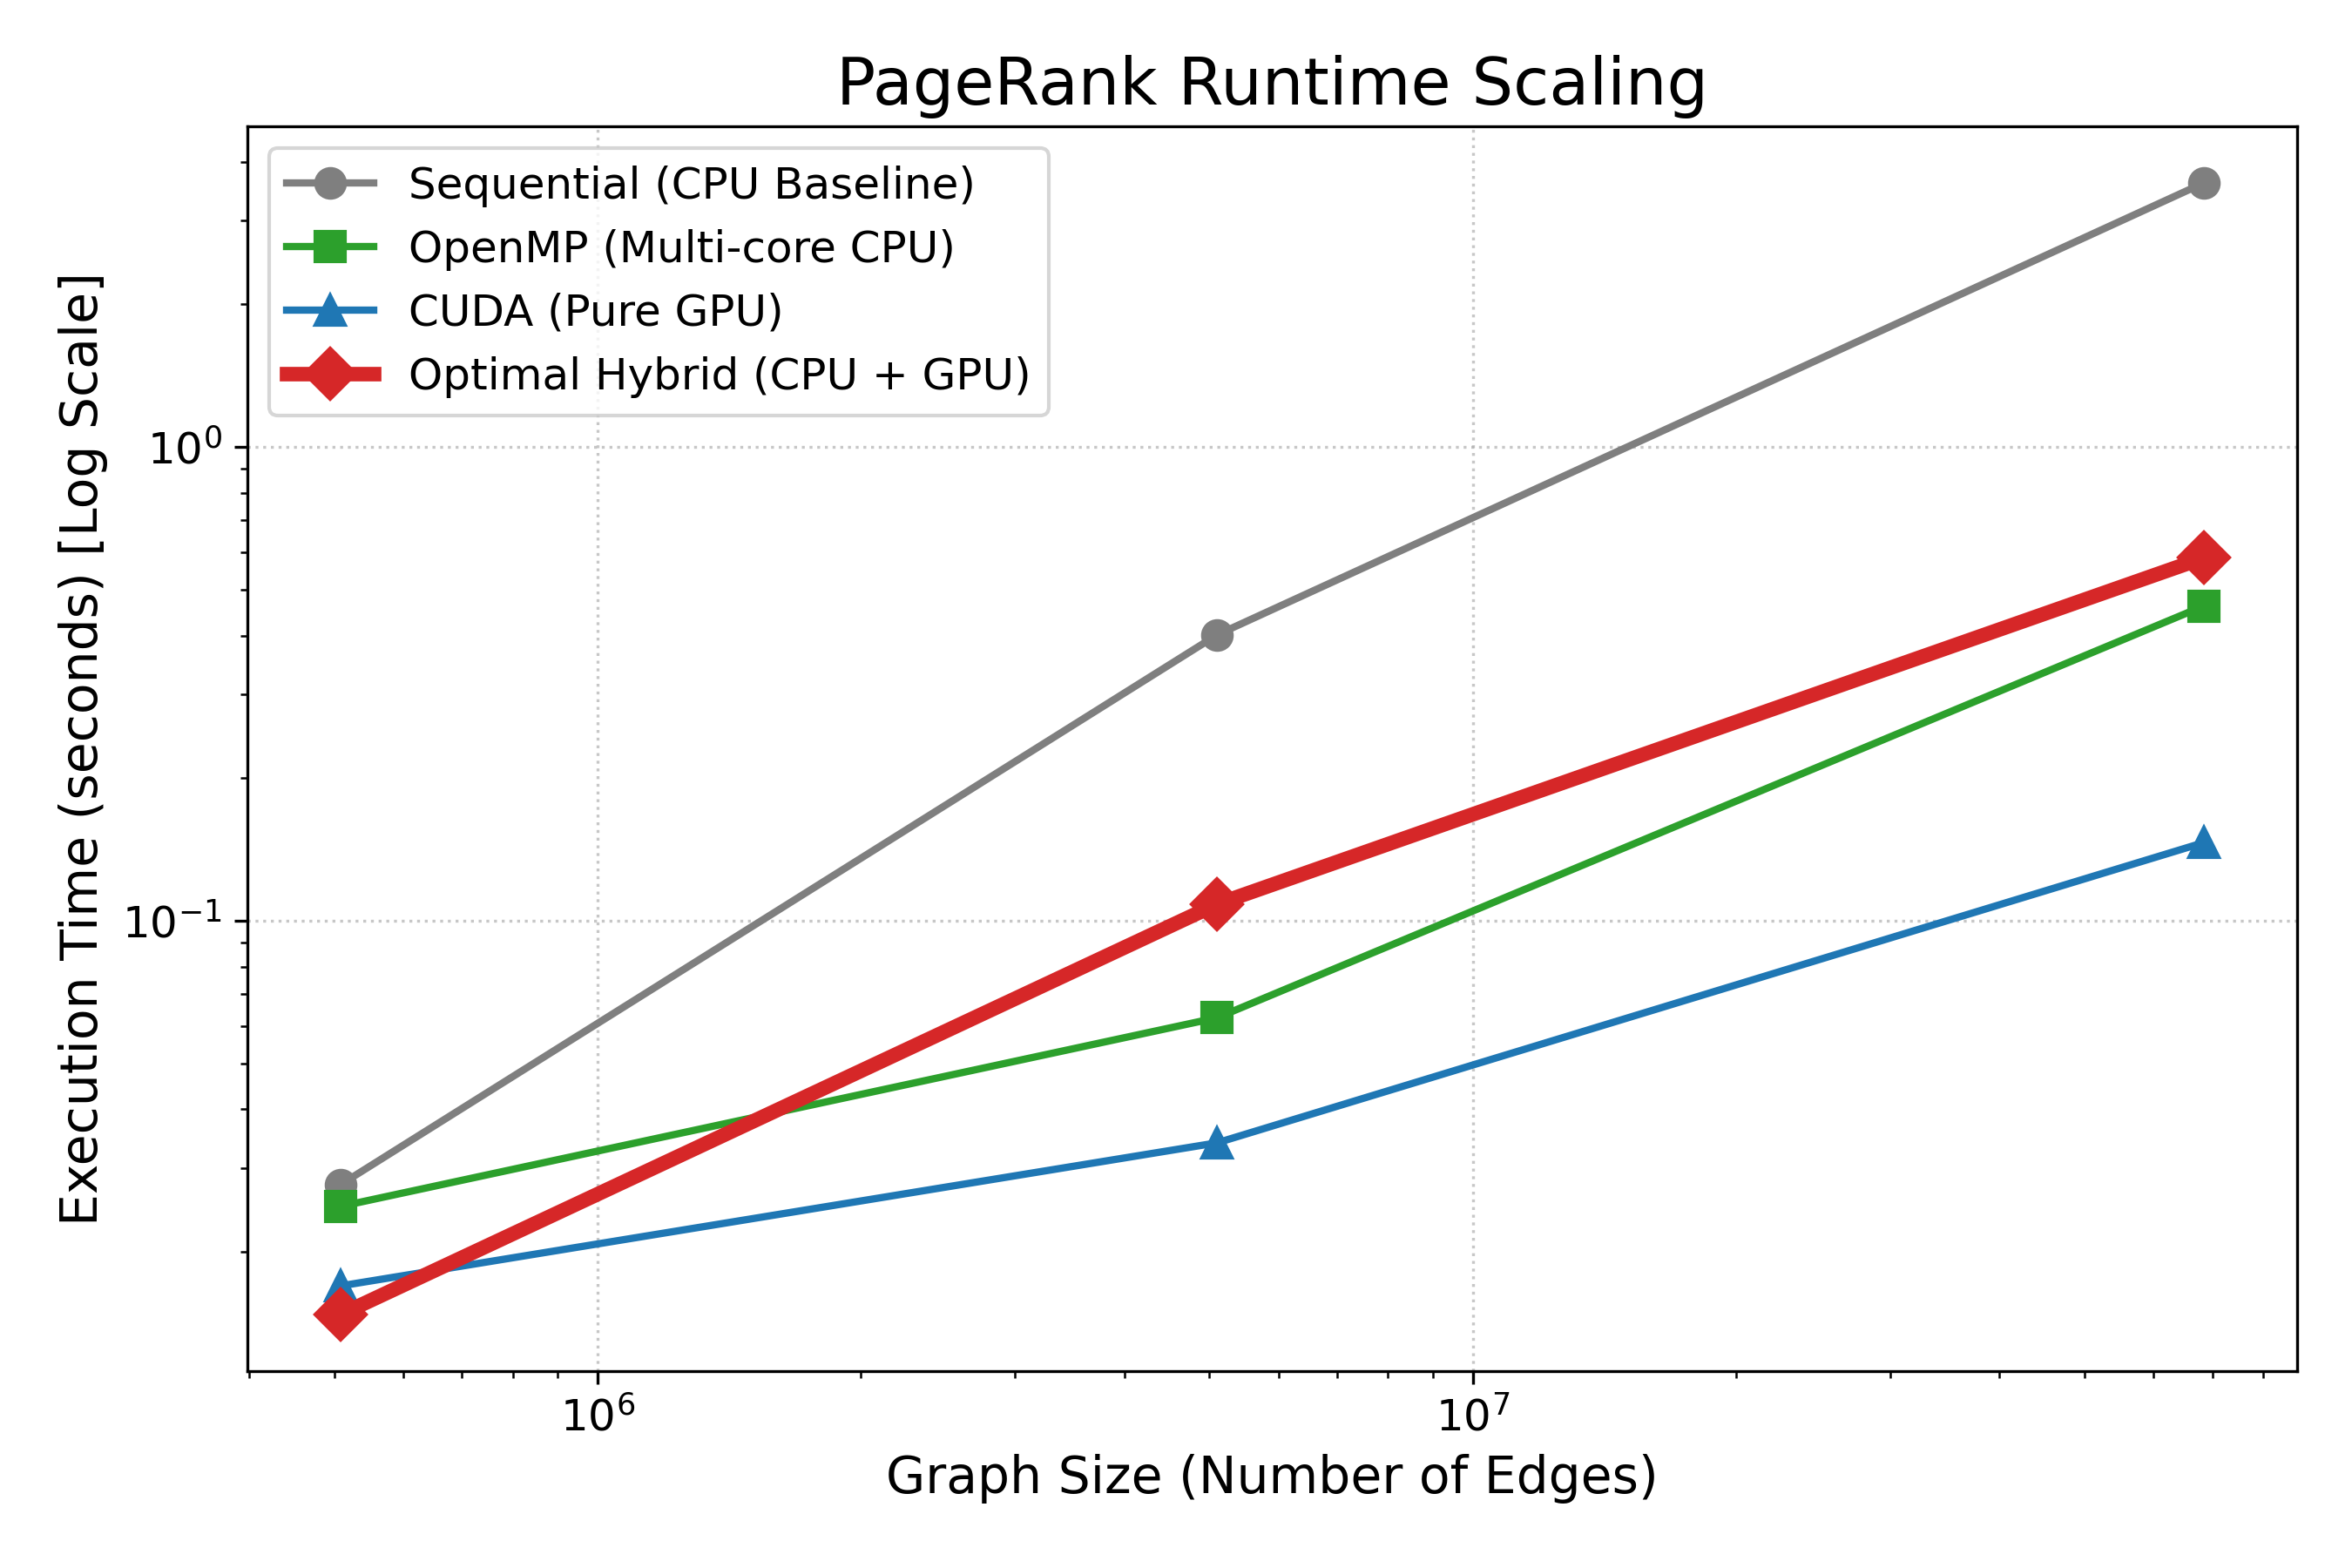
\includegraphics[width=\textwidth]{runtime.png}
           }{
               \rule{\textwidth}{5.5cm} % Placeholder if image isn't available in preview
           }
           \caption{Execution Time vs Graph Size}
           \label{fig:runtime}
       \end{subfigure}
       \hfill
       \begin{subfigure}[b]{0.48\textwidth}
           \centering
           \IfFileExists{speedup.png}{
               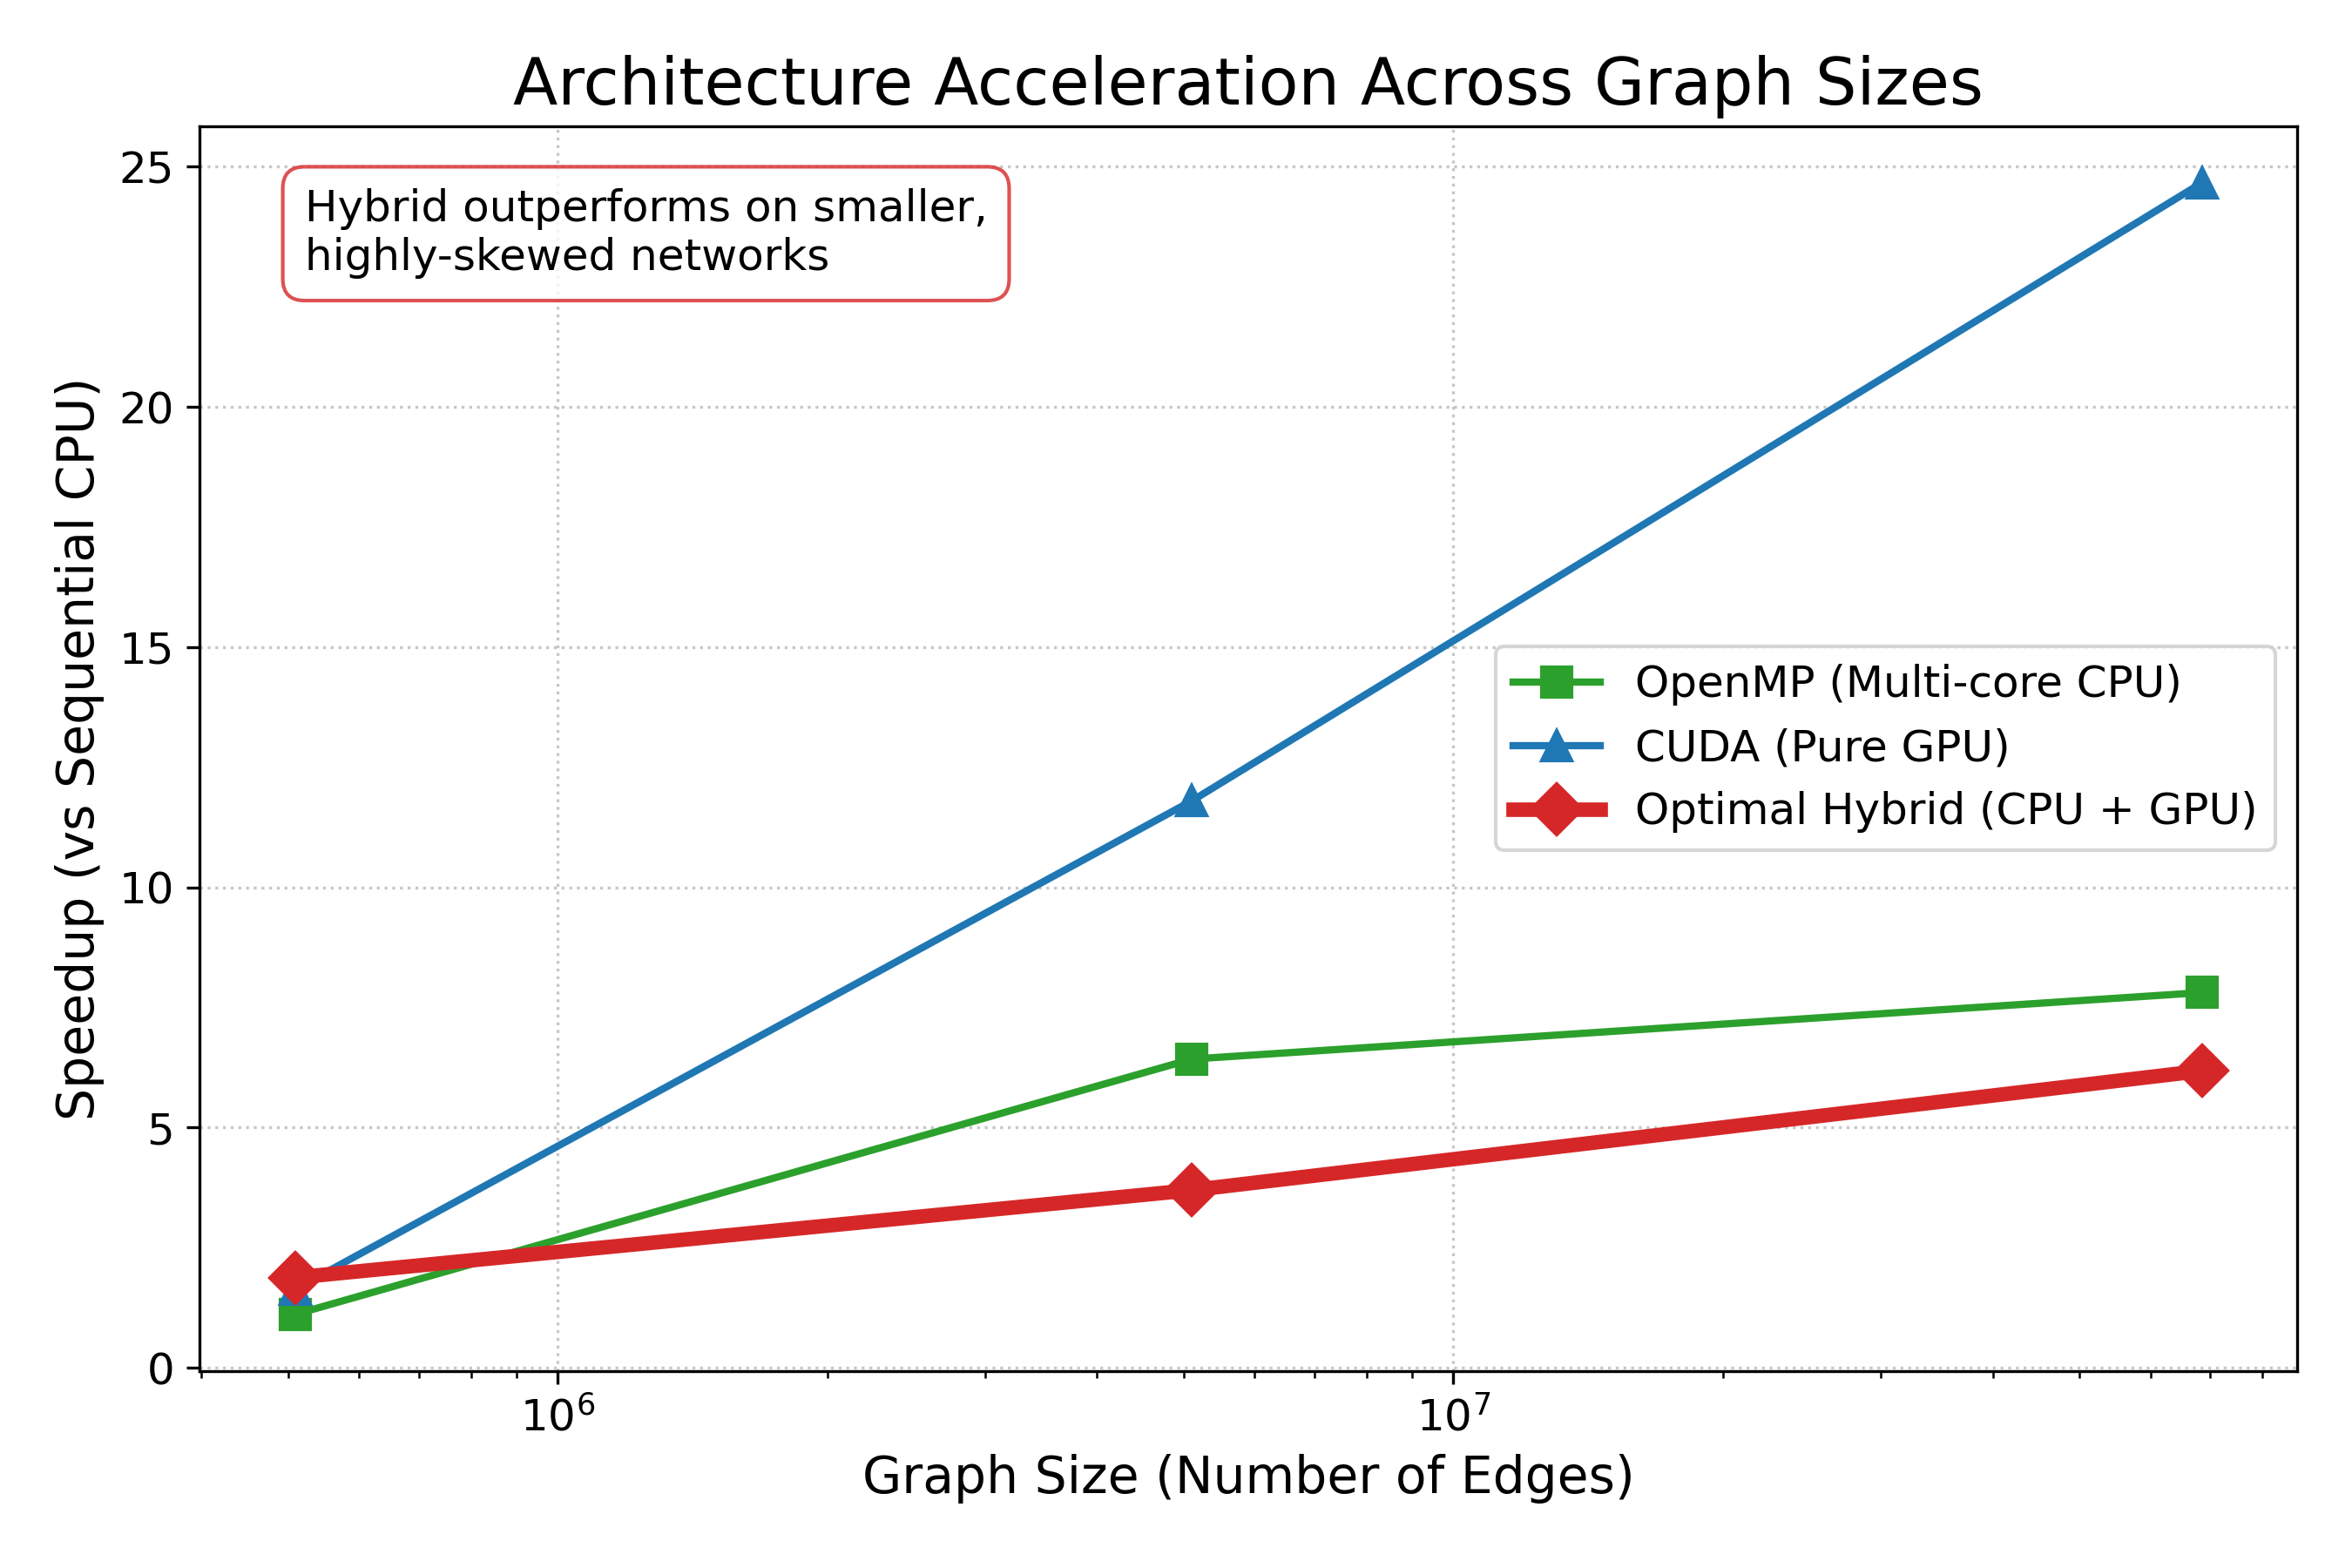
\includegraphics[width=\textwidth]{speedup.png}
           }{
               \rule{\textwidth}{5.5cm} % Placeholder if image isn't available in preview
           }
           \caption{Speedup vs Sequential Baseline}
           \label{fig:speedup}
       \end{subfigure}
       \caption{Performance scaling of the PageRank engines. The Hybrid approach demonstrates superior acceleration on smaller, highly-skewed networks, while Pure CUDA scaling dominates exponentially at massive sizes.}
       \label{fig:scaling_charts}
   \end{figure}
   
   The parameter sweep across the dataset and the visualizations reveal three distinct hardware realities:

   \paragraph{1. The ``Sweet Spot'' (Warp Divergence Mitigated)}
   On smaller, highly-skewed graphs (\texttt{soc-Epinions}), the Hybrid engine successfully outperforms both OpenMP and Pure CUDA, achieving a \textbf{2.05$\times$} speedup (as seen in Figure \ref{fig:speedup}). By routing the top 2\% of hubs to the CPU, warp divergence was eliminated. Because the graph's overall memory footprint is small, the PCIe transfer latency was negligible, allowing the CPU computation to perfectly overlap and hide the memory transfer cost.

   \paragraph{2. The Starvation Penalty}
   When the high-degree threshold is set too low (e.g., $hd=0.05\%$), the CPU is starved of work. Assigning only a few dozen vertices to the CPU means the latency of spawning OpenMP threads outweighs the computational benefit, dropping efficiency significantly.

   \paragraph{3. The PCIe Floor}
   On massive datasets (\texttt{soc-LiveJournal}), Pure CUDA heavily dominates (24.66$\times$ speedup). In large graphs, the rank array becomes massive (e.g., 19.3 MB). Transferring this array back and forth across the PCIe bus every iteration establishes a hard time constraint. Despite utilizing pinned memory and asynchronous streams, doing 50 round-trips over the PCIe bus limits the Hybrid engine to $\sim0.58$ seconds, while the Pure GPU engine (computing entirely inside 500+ GB/s VRAM) finishes the entire workload in $0.14$ seconds.

   \section{Conclusion}
   We successfully engineered an asynchronous heterogeneous CPU-GPU solver for PageRank. By utilizing pinned memory and CUDA streams, the architecture perfectly overlaps CPU computation with GPU data transfers. 
    
   The results prove that routing high-degree hubs to the CPU effectively eliminates GPU warp divergence, allowing the Hybrid engine to achieve peak efficiency on skewed networks. However, benchmarking also identified a hard physical limit on web-scale graphs: Pure GPU execution dominates massive datasets because bypassing PCIe bandwidth limits is ultimately more impactful than mitigating warp divergence. Future scaling requires leveraging unified memory architectures (NVLink) or distributed multi-GPU environments (NCCL).

	\newpage
	\addcontentsline{toc}{section}{References}
	\IfFileExists{mybib.bib}{
	    \bibliographystyle{IEEEtran}
	    \bibliography{mybib}
	}{}
  
\end{document}